\documentclass{article}
\usepackage[a4paper, total={16cm, 25cm}]{geometry}
\usepackage{amsfonts}
\usepackage{graphicx} % Required for inserting images
\usepackage{listings}
\usepackage[fleqn]{amsmath}
\usepackage{amssymb}
\usepackage{systeme}
\usepackage{xcolor}
\usepackage{float}
\usepackage{tikz}

\usetikzlibrary{decorations.pathmorphing}
\usetikzlibrary{fadings}

\title{Memo about a certain exam question}
\author{David Ferreira de Sousa Duque}
\date{February 2023}

\definecolor{bgc}{rgb}{0.975,0.975,0.975}
\definecolor{taskA}{rgb}{0.8,0.2,0.8}
\definecolor{taskC}{rgb}{0.2,0.2,1}
\definecolor{taskB}{rgb}{0.4,0.4,0.4}

\lstdefinestyle{default}{
    backgroundcolor=\color{bgc},
    numbers = left
}
\lstset{style=default}

\allowdisplaybreaks

\begin{document}

\maketitle

\section{The Question}
\paragraph{}

An application has a modified round-robin with interrupts pattern composed by 3 tasks - \textbf{A}, \textbf{B} and \textbf{C}:
\begin{lstlisting}
loop {
    if (serve_A OR serve_C) {
        A(); B(); C();
    }
}
\end{lstlisting}

In the original problem, there was an else block that was commented, so it's not considered here.

A(), B() and C() are all defined as follows:
\begin{lstlisting}
A() {
    if (serve_A) {
        serve_A = FALSE;
        DoTask(A);
    }
}

C() {
    if (serve_C) {
        serve_C = FALSE;
        DoTask(C);
    }
}

B() {
    DoTask(B);
}
\end{lstlisting}

This application has the following specifications:

\begin{table}[H]
\centering
 \begin{tabular}{||c | c | c||} 
 \hline
 Task & Service Time & Period \\ [0.5ex] 
 \hline\hline
 A & $300 \mu$s & $1000 \mu$s \\ 
 B & $? \mu$s & - \\
 C & $200 \mu$s & $1000 \mu$s \\ [1ex] 
 \hline
 \end{tabular}
\end{table}

We want to know what's the largest possible service time for \textbf{B} so that the tasks \textbf{A} and \textbf{C} are executed before they are requested again.

The rationale for a naturally thought-to-be correct answer involves that in a worst case scenario, \textbf{B} would be executed twice, therefore the maximum service time for it would be $250 \mu$s. ($300 + 250 + 250 + 200 = 1000$). But we want to prove that this maximum service time is actually $500 \mu$s.

\section{Assumptions}
\paragraph{}

The tasks \textbf{A} and \textbf{C} have a period of $1000 \mu$s. However, we cannot assume anything about whether the periods are synchronized or not, but we can still gather the following assumptions:

\begin{itemize}
  \item \textbf{A} and \textbf{C} have a repetition period of $1000 \mu$s;
  \item \textbf{A} is requested at $\{1000 \times n, n \in \mathbb{N}_1\}\text{ }\mu$s;
  \item \textbf{C} is requested at $\{1000 \times n + \mathbf{T}, n \in \mathbb{N}_1\}, \mathbf{T} \in \mathbf{]}-1000, 1000\mathbf{[}\text{ }\mu$s;
  \item The service time of \textbf{B}, $\mathbf{t_B} \in \mathbf{]}0, 500\mathbf{]}\text{ }\mu$s;
  \item The service time of \textbf{A} and \textbf{C} are equal to $\mathbf{t_A} = 300\mu$s and $\mathbf{t_C} = 200\mu$s, respectively
  \item The overhead caused by interrupts and service flag checking is negligible (i.e. irrelevant) for this problem; 
\end{itemize}

\section{Rationale \& Examples}
\paragraph{}

Let's consider the following timelines. These are not intended to be exhaustive, but instead intended to demonstrate various scenarios:

\subsection{A and C requested at the same time}

$$
\begin{cases}
    T = 0\\
    t_B = 500
\end{cases}
$$

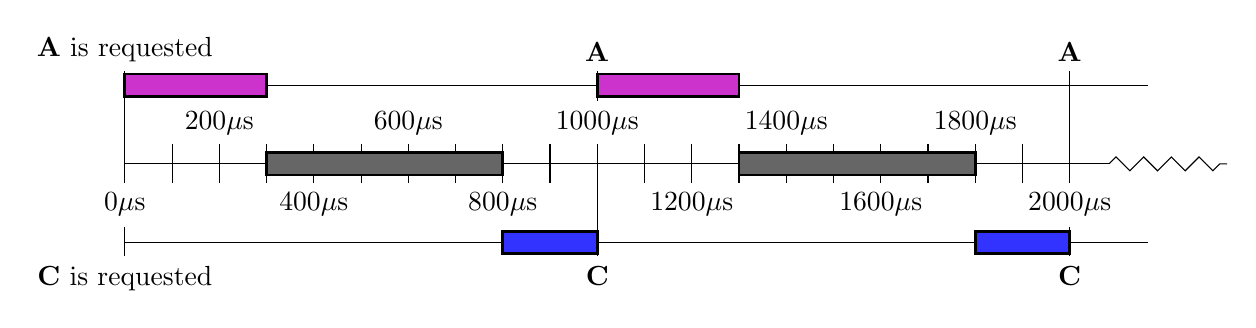
\begin{tikzpicture}[]
    % draw horizontal line   
    \draw (0,0) -- (12.5,0);
    \draw[decorate, decoration=zigzag] (12.5,0) -- (14,0);

    % draw vertical lines
    \foreach \x in {0,0.6,1.2,1.8,2.4,3,3.6,4.2,4.8,5.4,6,6.6,7.2,7.8,8.4,9,9.6,10.2,10.8,11.4,12}
    \draw (\x cm,7pt) -- (\x cm,-7pt);

    % draw nodes
    \draw (0.0,0) node[below=7pt] {$ 0 \mu$s};
    \draw (1.2,0) node[above=7pt] {$ 200 \mu$s};
    \draw (2.4,0) node[below=7pt] {$ 400 \mu$s};
    \draw (3.6,0) node[above=7pt] {$ 600 \mu$s};
    \draw (4.8,0) node[below=7pt] {$ 800 \mu$s};
    \draw (6.0,0) node[above=7pt] {$ 1000 \mu$s};
    \draw (7.2,0) node[below=7pt] {$ 1200 \mu$s};
    \draw (8.4,0) node[above=7pt] {$ 1400 \mu$s};
    \draw (9.6,0) node[below=7pt] {$ 1600 \mu$s};
    \draw (10.8,0) node[above=7pt] {$ 1800 \mu$s};
    \draw (12.0,0) node[below=7pt] {$ 2000 \mu$s};

    % Draw Service Timelines
    \draw (0, 1) -- (13, 1cm);
    \draw (0, 0) -- (0, 1cm + 5pt);
    \draw (6, 0.8) -- (6, 1cm + 5pt);
    \draw (12, 0) -- (12, 1cm + 5pt);
    \draw (0, 1cm) node[above=5pt] {\textbf{A} is requested};
    \draw (6, 1cm) node[above=5pt] {\textbf{A}};
    \draw (12, 1cm) node[above=5pt] {\textbf{A}};

    \draw (0, -1) -- (13, -1cm);
    \draw (0, -0.8) -- (0, -1cm - 5pt);
    \draw (6, 0) -- (6, -1cm - 5pt);
    \draw (12, -0.8) -- (12, -1cm - 5pt);
    \draw (0, -1cm) node[below=5pt] {\textbf{C} is requested};
    \draw (6, -1cm) node[below=5pt] {\textbf{C}};
    \draw (12, -1cm) node[below=5pt] {\textbf{C}};

    % Draw Task Executions
    \draw[color=black,line width=1pt,fill=taskA] (0.0,1cm + 4pt) -- (1.8,1cm + 4pt) -- (1.8,1cm - 4pt) -- (0.0,1cm - 4pt) -- cycle;
    \draw[color=black,line width=1pt,fill=taskA] (6.0,1cm + 4pt) -- (7.8,1cm + 4pt) -- (7.8,1cm - 4pt) -- (6.0,1cm - 4pt) -- cycle;

    \draw[color=black,line width=1pt,fill=taskB] (1.8,4pt) -- (4.8,4pt) -- (4.8,-4pt) -- (1.8,-4pt) -- cycle;
    \draw[color=black,line width=1pt,fill=taskB] (7.8,4pt) -- (10.8,4pt) -- (10.8,-4pt) -- (7.8,-4pt) -- cycle;

    \draw[color=black,line width=1pt,fill=taskC] (4.8,-1cm + 4pt) -- (6.0,-1cm + 4pt) -- (6.0,-1cm - 4pt) -- (4.8,-1cm - 4pt) -- cycle;
    \draw[color=black,line width=1pt,fill=taskC] (10.8,-1cm + 4pt) -- (12.0,-1cm + 4pt) -- (12.0,-1cm - 4pt) -- (10.8,-1cm - 4pt) -- cycle;
\end{tikzpicture}

In this case, the useful load is 100\%. Since both \textbf{A} and \textbf{C} are requested at the same time, \textbf{B} only runs once per loop.

\subsection{C requested after A, but before B ends}

$$
\begin{cases}
    T = 500\\
    t_B = 500
\end{cases}
$$

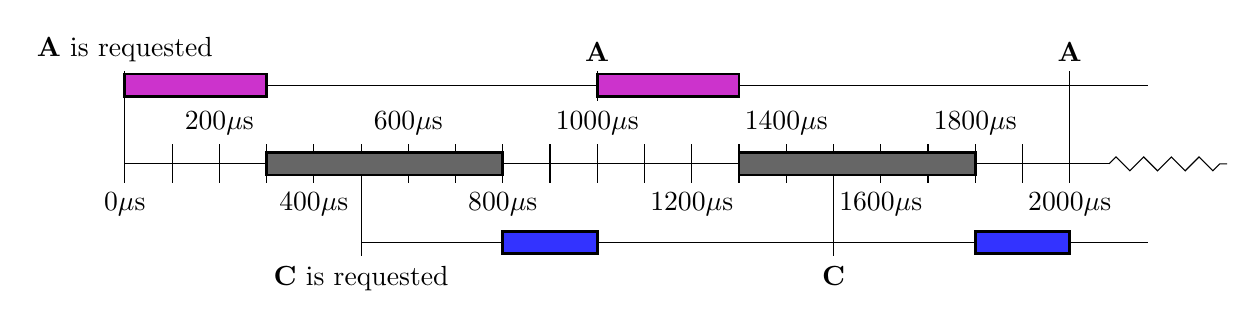
\begin{tikzpicture}[]
    % draw horizontal line   
    \draw (0,0) -- (12.5,0);
    \draw[decorate, decoration=zigzag] (12.5,0) -- (14,0);

    % draw vertical lines
    \foreach \x in {0,0.6,1.2,1.8,2.4,3,3.6,4.2,4.8,5.4,6,6.6,7.2,7.8,8.4,9,9.6,10.2,10.8,11.4,12}
        \draw (\x cm,7pt) -- (\x cm,-7pt);

    % draw nodes
    \draw (0.0,0) node[below=7pt] {$ 0 \mu$s};
    \draw (1.2,0) node[above=7pt] {$ 200 \mu$s};
    \draw (2.4,0) node[below=7pt] {$ 400 \mu$s};
    \draw (3.6,0) node[above=7pt] {$ 600 \mu$s};
    \draw (4.8,0) node[below=7pt] {$ 800 \mu$s};
    \draw (6.0,0) node[above=7pt] {$ 1000 \mu$s};
    \draw (7.2,0) node[below=7pt] {$ 1200 \mu$s};
    \draw (8.4,0) node[above=7pt] {$ 1400 \mu$s};
    \draw (9.6,0) node[below=7pt] {$ 1600 \mu$s};
    \draw (10.8,0) node[above=7pt] {$ 1800 \mu$s};
    \draw (12.0,0) node[below=7pt] {$ 2000 \mu$s};

    % Draw Service Timelines
    \draw (0, 1) -- (13, 1cm);
    \draw (0, 0) -- (0, 1cm + 5pt);
    \draw (6, 0.8) -- (6, 1cm + 5pt);
    \draw (12, 0) -- (12, 1cm + 5pt);
    \draw (0, 1cm) node[above=5pt] {\textbf{A} is requested};
    \draw (6, 1cm) node[above=5pt] {\textbf{A}};
    \draw (12, 1cm) node[above=5pt] {\textbf{A}};

    \draw (3, -1) -- (13, -1cm);
    \draw (3, 0) -- (3, -1cm - 5pt);
    \draw (9, 0) -- (9, -1cm - 5pt);
    %\draw (12, -0.8) -- (12, -1cm - 5pt);
    \draw (3, -1cm) node[below=5pt] {\textbf{C} is requested};
    \draw (9, -1cm) node[below=5pt] {\textbf{C}};
    %\draw (12, -1cm) node[below=5pt] {\textbf{C}};

    % Draw Task Executions
    \draw[color=black,line width=1pt,fill=taskA] (0.0,1cm + 4pt) -- (1.8,1cm + 4pt) -- (1.8,1cm - 4pt) -- (0.0,1cm - 4pt) -- cycle;
    \draw[color=black,line width=1pt,fill=taskA] (6.0,1cm + 4pt) -- (7.8,1cm + 4pt) -- (7.8,1cm - 4pt) -- (6.0,1cm - 4pt) -- cycle;

    \draw[color=black,line width=1pt,fill=taskB] (1.8,4pt) -- (4.8,4pt) -- (4.8,-4pt) -- (1.8,-4pt) -- cycle;
    \draw[color=black,line width=1pt,fill=taskB] (7.8,4pt) -- (10.8,4pt) -- (10.8,-4pt) -- (7.8,-4pt) -- cycle;

    \draw[color=black,line width=1pt,fill=taskC] (4.8,-1cm + 4pt) -- (6.0,-1cm + 4pt) -- (6.0,-1cm - 4pt) -- (4.8,-1cm - 4pt) -- cycle;
    \draw[color=black,line width=1pt,fill=taskC] (10.8,-1cm + 4pt) -- (12.0,-1cm + 4pt) -- (12.0,-1cm - 4pt) -- (10.8,-1cm - 4pt) -- cycle;
\end{tikzpicture}

Here, \textbf{C} is on the opposite phase of \textbf{A}. However, by the time it is requested, \textbf{B} didn't finish executing yet, and therefore the loop will not repeat. \textbf{B} does not repeat and both \textbf{A} and \textbf{C} have their service deadlines satisfied.

\subsection{C requested after A and after B ends}

$$
\begin{cases}
    T = 850\\
    t_B = 500
\end{cases}
$$

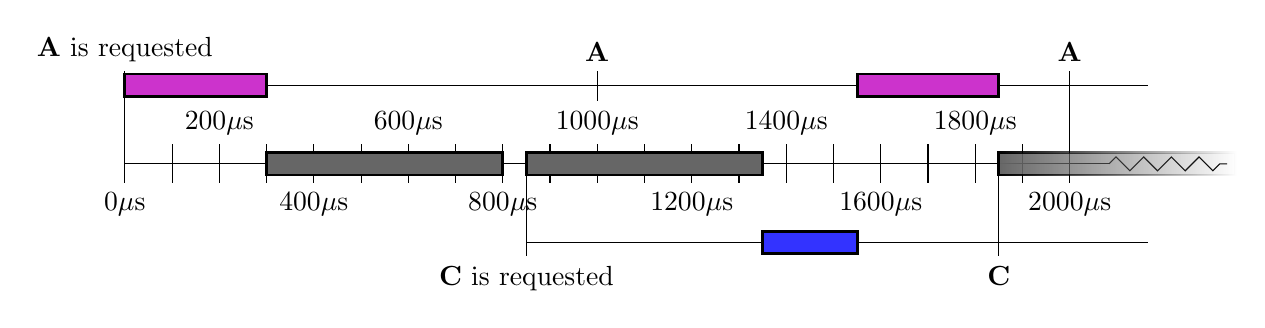
\begin{tikzpicture}[]
    % draw horizontal line   
    \draw (0,0) -- (12.5,0);
    \draw[decorate, decoration=zigzag] (12.5,0) -- (14,0);

    % draw vertical lines
    \foreach \x in {0,0.6,1.2,1.8,2.4,3,3.6,4.2,4.8,5.4,6,6.6,7.2,7.8,8.4,9,9.6,10.2,10.8,11.4,12}
        \draw (\x cm,7pt) -- (\x cm,-7pt);

    % draw nodes
    \draw (0.0,0) node[below=7pt] {$ 0 \mu$s};
    \draw (1.2,0) node[above=7pt] {$ 200 \mu$s};
    \draw (2.4,0) node[below=7pt] {$ 400 \mu$s};
    \draw (3.6,0) node[above=7pt] {$ 600 \mu$s};
    \draw (4.8,0) node[below=7pt] {$ 800 \mu$s};
    \draw (6.0,0) node[above=7pt] {$ 1000 \mu$s};
    \draw (7.2,0) node[below=7pt] {$ 1200 \mu$s};
    \draw (8.4,0) node[above=7pt] {$ 1400 \mu$s};
    \draw (9.6,0) node[below=7pt] {$ 1600 \mu$s};
    \draw (10.8,0) node[above=7pt] {$ 1800 \mu$s};
    \draw (12.0,0) node[below=7pt] {$ 2000 \mu$s};

    % Draw Service Timelines
    \draw (0, 1) -- (13, 1cm);
    \draw (0, 0) -- (0, 1cm + 5pt);
    \draw (6, 0.8) -- (6, 1cm + 5pt);
    \draw (12, 0) -- (12, 1cm + 5pt);
    \draw (0, 1cm) node[above=5pt] {\textbf{A} is requested};
    \draw (6, 1cm) node[above=5pt] {\textbf{A}};
    \draw (12, 1cm) node[above=5pt] {\textbf{A}};

    \draw (5.1, -1) -- (13, -1cm);
    \draw (5.1, 0) -- (5.1, -1cm - 5pt);
    \draw (11.1, 0) -- (11.1, -1cm - 5pt);
    %\draw (12, -0.8) -- (12, -1cm - 5pt);
    \draw (5.1, -1cm) node[below=5pt] {\textbf{C} is requested};
    \draw (11.1, -1cm) node[below=5pt] {\textbf{C}};
    %\draw (12, -1cm) node[below=5pt] {\textbf{C}};

    % Draw Task Executions
    \draw[color=black,line width=1pt,fill=taskA] (0.0,1cm + 4pt) -- (1.8,1cm + 4pt) -- (1.8,1cm - 4pt) -- (0.0,1cm - 4pt) -- cycle;
    \draw[color=black,line width=1pt,fill=taskA] (9.3,1cm + 4pt) -- (11.1,1cm + 4pt) -- (11.1,1cm - 4pt) -- (9.3,1cm - 4pt) -- cycle;

    \draw[color=black,line width=1pt,fill=taskB] (1.8,4pt) -- (4.8,4pt) -- (4.8,-4pt) -- (1.8,-4pt) -- cycle;
    \draw[color=black,line width=1pt,fill=taskB] (5.1,4pt) -- (8.1,4pt) -- (8.1,-4pt) -- (5.1,-4pt) -- cycle;
    \draw[color=black,line width=1pt,fill=taskB,path fading=east] (11.1,4pt) -- (14.1,4pt) -- (14.1,-4pt) -- (11.1,-4pt) -- cycle;

    \draw[color=black,line width=1pt,fill=taskC] (8.1,-1cm + 4pt) -- (9.3,-1cm + 4pt) -- (9.3,-1cm - 4pt) -- (8.1,-1cm - 4pt) -- cycle;
\end{tikzpicture}

In this particular case, since \textbf{C} was requested after \textbf{B} has completed, the loop demands \textbf{B} to be ran again. But after that, we enter in a cycle: every time \textbf{C} is requested, \textbf{B} runs, then \textbf{C}, and finally ending in \textbf{A}. At that point, \textbf{C} is requested again, but has to wait until \textbf{B} finishes first. This loop is out of phase, but there are still no service faults.

\subsection{C requested before A}

$$
\begin{cases}
    T = -400\\
    t_B = 500
\end{cases}
$$

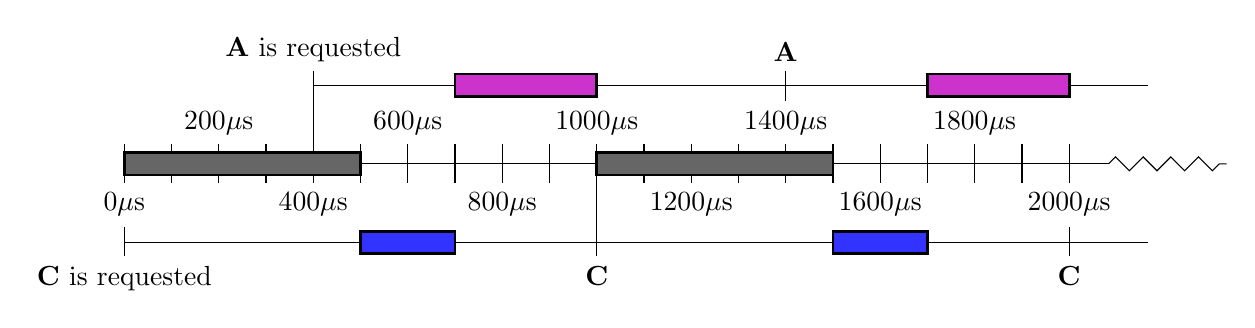
\begin{tikzpicture}[]
    % draw horizontal line
    \draw (0,0) -- (12.5,0);
    \draw[decorate, decoration=zigzag] (12.5,0) -- (14,0);

    % draw vertical lines
    \foreach \x in {0,0.6,1.2,1.8,2.4,3,3.6,4.2,4.8,5.4,6,6.6,7.2,7.8,8.4,9,9.6,10.2,10.8,11.4,12}
        \draw (\x cm,7pt) -- (\x cm,-7pt);

    % draw nodes
    \draw (0.0,0) node[below=7pt] {$ 0 \mu$s};
    \draw (1.2,0) node[above=7pt] {$ 200 \mu$s};
    \draw (2.4,0) node[below=7pt] {$ 400 \mu$s};
    \draw (3.6,0) node[above=7pt] {$ 600 \mu$s};
    \draw (4.8,0) node[below=7pt] {$ 800 \mu$s};
    \draw (6.0,0) node[above=7pt] {$ 1000 \mu$s};
    \draw (7.2,0) node[below=7pt] {$ 1200 \mu$s};
    \draw (8.4,0) node[above=7pt] {$ 1400 \mu$s};
    \draw (9.6,0) node[below=7pt] {$ 1600 \mu$s};
    \draw (10.8,0) node[above=7pt] {$ 1800 \mu$s};
    \draw (12.0,0) node[below=7pt] {$ 2000 \mu$s};

    % Draw Service Timelines
    \draw (2.4, 1) -- (13, 1cm);
    \draw (2.4, 0) -- (2.4, 1cm + 5pt);
    \draw (8.4, 0.8) -- (8.4, 1cm + 5pt);
    %\draw (12, 0) -- (12, 1cm + 5pt);
    \draw (2.4, 1cm) node[above=5pt] {\textbf{A} is requested};
    \draw (8.4, 1cm) node[above=5pt] {\textbf{A}};
    %\draw (12, 1cm) node[above=5pt] {\textbf{A}};

    \draw (0, -1) -- (13, -1cm);
    \draw (0, -0.8) -- (0, -1cm - 5pt);
    \draw (6, 0) -- (6, -1cm - 5pt);
    \draw (12, -0.8) -- (12, -1cm - 5pt);
    \draw (0, -1cm) node[below=5pt] {\textbf{C} is requested};
    \draw (6, -1cm) node[below=5pt] {\textbf{C}};
    \draw (12, -1cm) node[below=5pt] {\textbf{C}};

    % Draw Task Executions
    \draw[color=black,line width=1pt,fill=taskA] (4.2,1cm + 4pt) -- (6,1cm + 4pt) -- (6,1cm - 4pt) -- (4.2,1cm - 4pt) -- cycle;
    \draw[color=black,line width=1pt,fill=taskA] (10.2,1cm + 4pt) -- (12,1cm + 4pt) -- (12,1cm - 4pt) -- (10.2,1cm - 4pt) -- cycle;

    \draw[color=black,line width=1pt,fill=taskB] (0,4pt) -- (3,4pt) -- (3,-4pt) -- (0,-4pt) -- cycle;
    \draw[color=black,line width=1pt,fill=taskB] (6,4pt) -- (9,4pt) -- (9,-4pt) -- (6,-4pt) -- cycle;

    \draw[color=black,line width=1pt,fill=taskC] (3,-1cm + 4pt) -- (4.2,-1cm + 4pt) -- (4.2,-1cm - 4pt) -- (3,-1cm - 4pt) -- cycle;
    \draw[color=black,line width=1pt,fill=taskC] (9,-1cm + 4pt) -- (10.2,-1cm + 4pt) -- (10.2,-1cm - 4pt) -- (9,-1cm - 4pt) -- cycle;
\end{tikzpicture}

$$
\begin{cases}
    T = -800\\
    t_B = 500
\end{cases}
$$

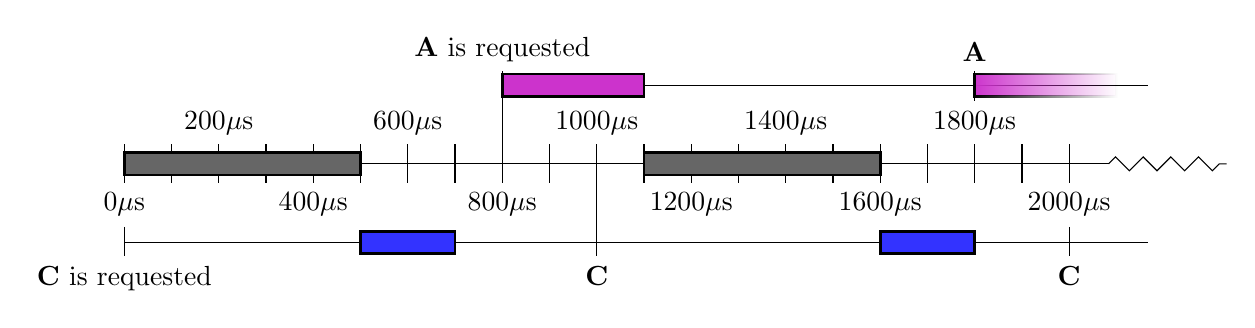
\begin{tikzpicture}[]
    % draw horizontal line
    \draw (0,0) -- (12.5,0);
    \draw[decorate, decoration=zigzag] (12.5,0) -- (14,0);

    % draw vertical lines
    \foreach \x in {0,0.6,1.2,1.8,2.4,3,3.6,4.2,4.8,5.4,6,6.6,7.2,7.8,8.4,9,9.6,10.2,10.8,11.4,12}
        \draw (\x cm,7pt) -- (\x cm,-7pt);

    % draw nodes
    \draw (0.0,0) node[below=7pt] {$ 0 \mu$s};
    \draw (1.2,0) node[above=7pt] {$ 200 \mu$s};
    \draw (2.4,0) node[below=7pt] {$ 400 \mu$s};
    \draw (3.6,0) node[above=7pt] {$ 600 \mu$s};
    \draw (4.8,0) node[below=7pt] {$ 800 \mu$s};
    \draw (6.0,0) node[above=7pt] {$ 1000 \mu$s};
    \draw (7.2,0) node[below=7pt] {$ 1200 \mu$s};
    \draw (8.4,0) node[above=7pt] {$ 1400 \mu$s};
    \draw (9.6,0) node[below=7pt] {$ 1600 \mu$s};
    \draw (10.8,0) node[above=7pt] {$ 1800 \mu$s};
    \draw (12.0,0) node[below=7pt] {$ 2000 \mu$s};

    % Draw Service Timelines
    \draw (4.8, 1) -- (13, 1cm);
    \draw (4.8, 0) -- (4.8, 1cm + 5pt);
    \draw (10.8, 0.8) -- (10.8, 1cm + 5pt);
    %\draw (12, 0) -- (12, 1cm + 5pt);
    \draw (4.8, 1cm) node[above=5pt] {\textbf{A} is requested};
    \draw (10.8, 1cm) node[above=5pt] {\textbf{A}};
    %\draw (12, 1cm) node[above=5pt] {\textbf{A}};

    \draw (0, -1) -- (13, -1cm);
    \draw (0, -0.8) -- (0, -1cm - 5pt);
    \draw (6, 0) -- (6, -1cm - 5pt);
    \draw (12, -0.8) -- (12, -1cm - 5pt);
    \draw (0, -1cm) node[below=5pt] {\textbf{C} is requested};
    \draw (6, -1cm) node[below=5pt] {\textbf{C}};
    \draw (12, -1cm) node[below=5pt] {\textbf{C}};

    % Draw Task Executions
    \draw[color=black,line width=1pt,fill=taskA] (4.8, 1cm + 4pt) -- (6.6, 1cm + 4pt) -- (6.6, 1cm - 4pt) -- (4.8, 1cm - 4pt) -- cycle;
    \draw[color=black,line width=1pt,fill=taskA,path fading=east] (10.8, 1cm + 4pt) -- (12.6, 1cm + 4pt) -- (12.6, 1cm - 4pt) -- (10.8, 1cm - 4pt) -- cycle;

    \draw[color=black,line width=1pt,fill=taskB] (0, 4pt) -- (3,4pt) -- (3,-4pt) -- (0,-4pt) -- cycle;
    \draw[color=black,line width=1pt,fill=taskB] (6.6, 4pt) -- (9.6, 4pt) -- (9.6, -4pt) -- (6.6, -4pt) -- cycle;

    \draw[color=black,line width=1pt,fill=taskC] (3,-1cm + 4pt) -- (4.2,-1cm + 4pt) -- (4.2,-1cm - 4pt) -- (3,-1cm - 4pt) -- cycle;
    \draw[color=black,line width=1pt,fill=taskC] (9.6, -1cm + 4pt) -- (10.8,-1cm + 4pt) -- (10.8,-1cm - 4pt) -- (9.6,-1cm - 4pt) -- cycle;
\end{tikzpicture}

This pattern is analogue to the one seen in \textbf{3.3}. When \textbf{A} is requested after the first \textbf{B} task is completed, it then continues on a pattern similar to the one seen in \textbf{3.2}.

\section{Generalizing}

Given the patterns we've seen above, we can draw a few scenarios:

\begin{enumerate}
    \item $T \ge 0$, $T \le t_A + t_B$ (\textbf{C} requested \textbf{before} \textbf{A} and \textbf{B} finish, includes \textbf{A} and \textbf{C} being requested at the same time);
    \item $T < 0$, $T \ge -(t_B + t_C)$ (\textbf{A} requested \textbf{before} \textbf{B} and \textbf{C} finish);
    \item $T > 0$, $T > t_A + t_B$ (\textbf{C} requested \textbf{after} \textbf{A} and \textbf{B} finish);
    \item $T < 0$, $T < -(t_B + t_C)$ (\textbf{A} requested \textbf{after} \textbf{B} and \textbf{C} finish);
\end{enumerate}

Under any scenario, for any cycle $n \in \mathbb{N}_1$, the point in time where the tasks \textbf{A} and \textbf{C} are completed, $\tau_A$ and $\tau_C$ respectively, must follow the following inequation system:

$$
\begin{cases}
    1000n < \tau_A \le 1000(n+1)\\
    1000n + T < \tau_C \le 1000(n+1) + T
\end{cases}
$$

\subsection{$T \ge 0$, $T \le t_A + t_B$}

Under this scenario, for any given $n \in \mathbb{N}_1$:

\begin{flalign*}
\phantom{\iff}&\begin{cases}
    T > 0\\
    T \le t_A + t_B\\
    \tau_A = 1000n + t_A\\
    \tau_C = 1000n + t_A + t_B + t_C\\
    1000n < \tau_A \le 1000(n+1)\\
    1000n + T < \tau_C \le 1000(n+1) + T\\
\end{cases}\\
\iff&\begin{cases}
    1000n < 1000n + t_A \le 1000n + 1000\\
    1000n + T < 1000n + t_A + t_B + t_C \le 1000n + 1000 + T\\
\end{cases}\\
\iff&\begin{cases}
    0 < t_A \le 1000\\
    T < t_A + t_B + t_C \le 1000 + T\\
\end{cases}\\
\iff&\begin{cases}
    0 < 300 \le 1000\\
    T < 300 + t_B + 200 \le 1000 + T\\
\end{cases}\\
\iff&T < t_B + 500 \le 1000 + T\\
\iff&-500 + T < t_B \le 500 + T
\end{flalign*}

Since $t_B > 0$, $t_B \in ]0, 500 + T]\text{ }\mu$s so that no service faults occur (\textbf{in that cycle only}).
Naturally though, we have to abide by the rule that $t_A + t_B + t_C \le 1000 \iff t_B \le 500 \mu$s. Otherwise we'd be stealing time from the following cycles and a service fault would eventually occur.

Therefore, in this scenario, we can safely have $t_B \in ]0, 500]\text{ }\mu$s with no service faults.

$\hfill\blacksquare$

\subsection{$T < 0$, $T \ge -(t_B + t_C)$}

Under this scenario, \textbf{B} runs first, then \textbf{C} and finally \textbf{A}. For any given $n \in \mathbb{N}_1$:
\begin{flalign*}
\phantom{\iff} & \begin{cases}
    T < 0\\
    T \ge -(t_B + t_C)\\
    t_A + t_B + t_C \le 1000\\
    \tau_A = 1000n + T + t_B + t_C + t_A\\
    \tau_C = 1000n + T + t_B + t_C\\
    1000n < \tau_A \le 1000(n+1)\\
    1000n + T < \tau_C \le 1000(n+1) + T\\
\end{cases}\\
\iff & \begin{cases}
    1000n < 1000n + T + t_B + t_C + t_A \le 1000n + 1000\\
    1000n + T < 1000n + T + t_B + t_C \le 1000n + 1000 + T\\
\end{cases}\\
\iff & \begin{cases}
    0 < T + t_B + t_C + t_A \le 1000\\
    T < T + t_B + t_C       \le 1000 + T\\
\end{cases}\\
\iff & \begin{cases}
    0 < T + t_B + t_C + t_A \le 1000\\
    0 < t_B + t_C \le 1000\\
\end{cases}\\
\iff & \begin{cases}
    0 < T + t_B + 200 + 300 \le 1000\\
    0 < t_B + 200 \le 1000\\
\end{cases}\\
\iff & \begin{cases}
    0 < T + t_B + 500 \le 1000\\
    -200 < t_B \le 800\\
\end{cases}\\
\iff & \begin{cases}
    T \ge -(t_B + 200)\\
    t_A + t_B + t_C \le 1000\\
    -T < t_B + 500 \le 1000 - T\\
    -200 < t_B \le 800\\
\end{cases}\\
\iff & \begin{cases}
    T \ge -t_B - 200\\
    0 < t_B \le 500 & t_B\text{ } \text{is never negative or above } 500\mu\text{s}\\
    -T < t_B + 500 \le 1000 - T
\end{cases}\\
\iff & \begin{cases}
    0 < t_B \le 500\\
    -T \le t_B + 200\\
    -T < t_B + 500\\
    t_B + 500 \le 1000 - T
\end{cases}\\
\iff & \begin{cases}
    0 < t_B \le 500\\
    -T \le t_B + 200\\
    t_B + 200 \le 700 - T
\end{cases}\\
\iff & \begin{cases}
    0 < t_B \le 500\\
    -T \le t_B + 200 \le 700 - T
\end{cases}\\
\iff & \begin{cases}
    0 < t_B \le 500\\
    -200 - T \le t_B \le 500 - T
\end{cases}\\
\end{flalign*}

We have a bit to unpack here. We haven't yet proved that $t_B$ is safe when at $500\mu$s yet. However, we know that:

$$
\begin{cases}
    T < 0\\
    T \ge -(t_B + 200)\\
\end{cases}
$$

As an example, for a $t_B = 400$, then $T \in [-600, 0[\text{ }\mu$s. This allows us to define the function $f(t_B) = [-(t_B + 200), 0[$
We can now define two values such as the $-200 - T \le t_B \le 500 - T$ condition we've arrived to is the most restrictive possible (the "worst case scenarios"): 

$$
-200 - T \le t_B \le 500 - T \mathbf{\longrightarrow} -200 - inf\ f(t_B) \le t_B \le 500 - sup\ f(t_B)
$$
\begin{flalign*}
    & -200 - inf\ f(t_B) \le t_B \le 500 - sup\ f(t_B)\\        
    \iff & -200 -(-(t_B + 200)) \le t_B \le 500 - 0\\
    \iff & -200 + 200 + t_B \le t_B \le 500\\
    \iff & t_B \le t_B \le 500\\
    \iff & t_B \le 500
\end{flalign*}

$\hfill\blacksquare$

\subsection{$T > t_A + t_B$}

For this scenario, we need to split the problem in two:

\subsubsection{The first cycle}

The first cycle is a request to \textbf{A}, and then the system goes to sleep. Because the service deadline of \textbf{A} is of $1000\mu$s and $t_A + t_B \le 800\mu$s, there will never be a service fault on this cycle.

\subsubsection{Subsequent cycles}

On subsequent cycles, \textbf{C} is first called, then \textbf{A} is called. We can then assume a situation similar to \textbf{4.3} by considering $T^- = T - 1000$ instead:

\begin{flalign*}
\phantom{\iff} & \begin{cases}
    T > t_A + t_B\\
    T < 1000\\
    T^- = T - 1000
\end{cases}\\
\iff & \begin{cases}
    T^- > t_A + t_B - 1000\\
    T^- < 1000 - 1000
\end{cases}\\
\iff & \begin{cases}
    T^- > 300 + t_B - 1000\\
    T^- < 0
\end{cases}\\
\iff & \begin{cases}
    T^- \ge -(t_B + t_C) & \text{For } T^- \text{ to be considered under scenario } \textbf{4.2}\\
    T^- > -700 + t_B\\
    T^- < 0
\end{cases}\\
\implies & \begin{cases}
    -700 + t_B > -(t_B + t_C)\\
    T^- < 0
\end{cases}\\
\iff & \begin{cases}
    -700 + t_B > -t_B - 200\\
    T^- < 0
\end{cases}\\
\iff & \begin{cases}
    2t_B > 500\\
    T^- < 0
\end{cases}\\
\iff & \begin{cases}
    t_B > 250\\
    T^- < 0
\end{cases}\\
\end{flalign*}

If $t_B > 250\mu$s, then it is guaranteed that $T - 1000$ fits the criteria in the scenario \textbf{4.2}. From there, it is proven that under this scenario, $t_B \in ]0, 500]\text{ }\mu$s.
While for $t_B \le 250\mu$s there is the possibility of multiple repetitions occurring, it's already established that even if \textbf{B} always runs twice every cycle (the worst case scenario), service deadlines are still met.

$\hfill\blacksquare$

\subsection{$T < -(t_B + t_C)$}

This scenario is similar to the one discussed in \textbf{4.3}:

\subsubsection{The first cycle}

The first cycle is a request to \textbf{C}, executing \textbf{B}, then \textbf{C}, and then the system goes to sleep. Because the service deadline of \textbf{C} is of $1000\mu$s and $t_B + t_C \le 700\mu$s, there will never be a service fault on this cycle.

\subsubsection{Subsequent cycles}

On subsequent cycles, \textbf{A} is first called, then \textbf{C} is called. We can then assume a situation similar to \textbf{4.1} by considering $T^+ = T + 1000$ instead. The demonstration is analogue to the one done in \textbf{4.3}, so for brevity it will not be shown here.

\end{document}
